\documentclass[11pt, a4paper, oneside, article]{memoir}
% Setting for memoir
% Set the margins of the document
\setlrmarginsandblock{2cm}{2cm}{*}
\setulmarginsandblock{2cm}{*}{1}
\checkandfixthelayout
\captionnamefont{\bfseries\small}
\captiontitlefont{\small}
\DisemulatePackage{setspace}            % Make sure package is not ignored
%
\usepackage[german, english]{babel}     % Langauge setting
\usepackage[onehalfspacing]{setspace}   % Set the line spacing of the document
\usepackage[utf8]{inputenc}
\usepackage{graphicx}
\usepackage{wrapfig}                    % Wrapping text arround figures
\usepackage{amsmath}                    % Advanced mathsymbols
\usepackage{chemformula}                % Chemical formulas
\usepackage{pgfgantt}                   % GANTT charts
% Abbreviation glossary
\usepackage[acronym]{glossaries}        
\makeglossaries                         % Generate the glossary
% Bibliography with biblatex
\usepackage[citestyle=alphabetic,bibstyle=authoryear, citestyle=authoryear, maxbibnames=100, maxcitenames=2, sorting=ynt, backend=biber]{biblatex}
\addbibresource[location=local, datatype=bibtex]{atmo.bib}

\usepackage{csquotes, xpatch}
\usepackage{etex, etoolbox, keyval, ifthen, url} % Needed for chicago-style citations

\chapterstyle{bringhurst}               % Set style for memoir
\graphicspath{{pictures/}}              % Set graphics path

\newcommand{\pcite}[1]{\parencite{#1}}

\begin{document}
%Term definitions
% Standard command
%\gls{⟨label⟩}
% Capitalize first letter
%\Gls{⟨label⟩}
% Pluralize term
%\glspl{⟨label⟩}
%Capitalize and pluralize term
%\Glspl{⟨label⟩}

%\newacronym{}{}{}

% Acronyms
\newacronym{voc}{VOC}{Volatile Organic Compound}
\newacronym{bvoc}{BVOC}{Biogenic Volatile Organic Compound}
\newacronym{et}{ET}{evapotranspiration}
\newacronym{npp}{NPP}{Net Primary Production}
\newacronym{odina}{ODINA}{Ozone Damage Interference on Nutrient Allocation}
\newacronym{cuo}{CUO}{Cumulative Uptake of Ozone}
\newacronym{cesm}{CESM}{Community Earth System Model}
\newacronym{clm}{CLM}{Community Land Model}
\newacronym{cam}{CAM}{Community Atmosphere Model}
\newacronym{fun}{FUN}{Fixation and Update of Nitrogen}


\chapter{Research context}
Earth System Model history, missing links and knowledge gaps…

Ozone is an important trace gas in the atmosphere. In accordance with its effects and realm of occurence, we can distinguish the good (stratosphere), the bad (troposphere), and the ugly (ambient air) ozone. Here we shall focus on the connection and feedback between the bad and the ugly sides of ozone. Ozone is ranked third amongst the most potent climate forcers. It contributes to warming in the troposphere where it is produced as a secondary air pollutant in chemical cycles involving precursors such as \ch{CO} and \ch{NO_x} as well as hydrocarbons (\gls{voc}, \gls{bvoc}). Ozone is highly toxic and harmful to human health and many ecosystems. Despite a successful reduction of precursors in recent years leading to a stagnation of the upward trend in tropospheric ozone concentrations, there are indications that climate feedback on the uptake by land biosphere can hamper reaching the ultimate air quality goal \pcite{NCC:Lin2020}. In drought conditions, plants will limit their transpiration by closing their stomata. Uptake through plants’ stomata is considered one of the most effective removal pathways of ozone but large uncertainties in non-stomatal removal remain \pcite{RG:Clifton2020}. At the same time, a high uptake of ozone considerably affects photosynthetic and stomatal uptake capacities but differently strongly. Accounting for this, \cite{BGS:Lombardozzi2013} could explain observed variation in photosynthesis in global scales. Franz et al. (2021) show potential ozone damage on vegetation under climate change scenarios involving explicit modeling on the plant physiological level. These previous studies have not included an online atmospheric chemistry. Here, we want to combine the efforts of process understanding at the vegetation level into a fully coupled ESM with atmospheric chemistry and state-of-the-art nutrient limited carbon sequestration and study the feedback of ozone damage and thermal stress on air quality targets and climate.

\chapter{Research questions}

\begin{wrapfigure}[19]{R}[0pt]{0.5\textwidth}
  % R - floating; r - h! [narrow lines] <- reduce whitespace below
  \centering
  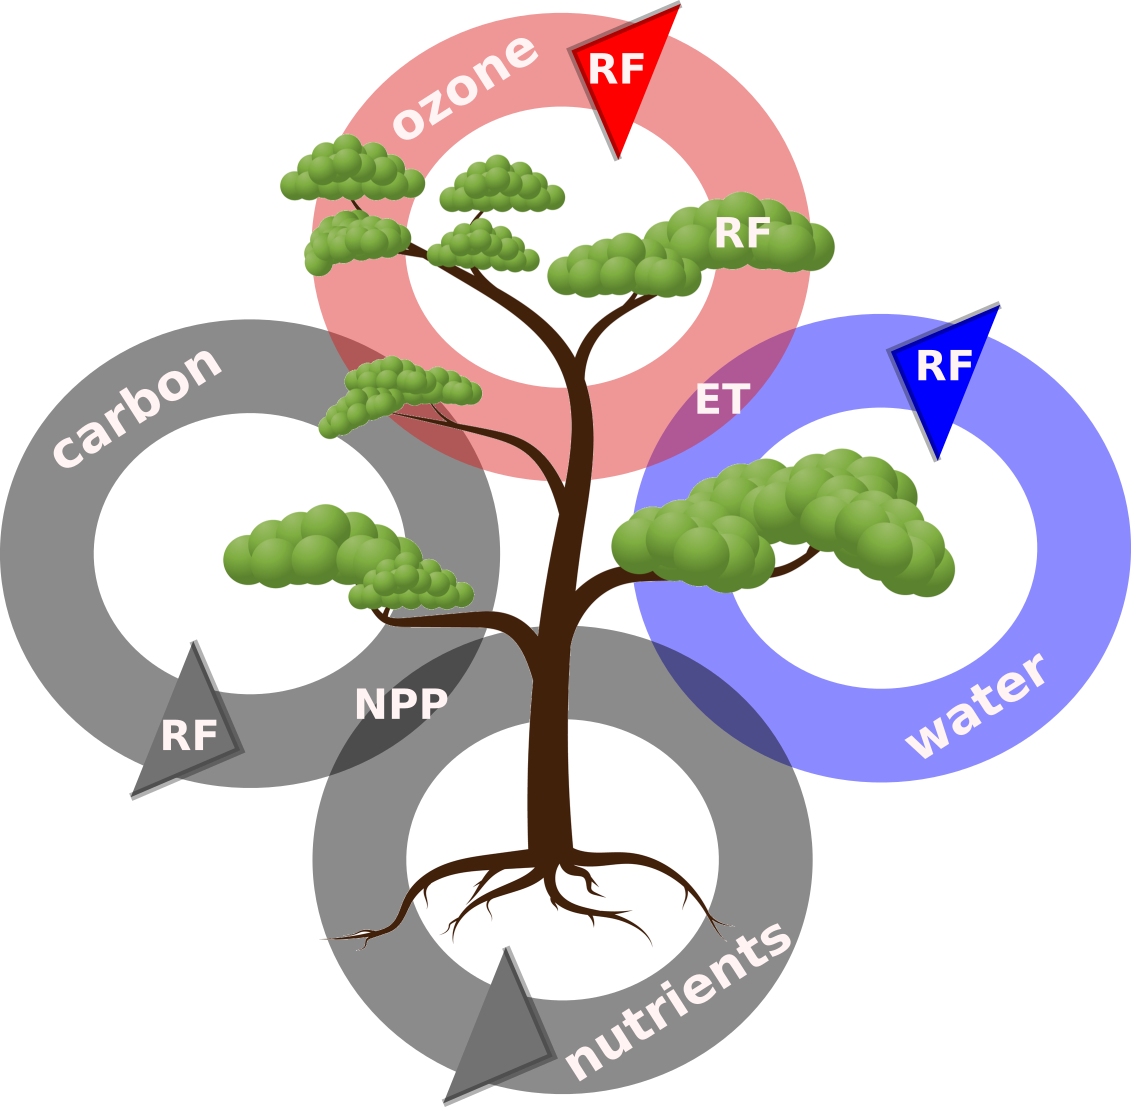
\includegraphics[width=0.48\textwidth]{ozone_es_scheme}
  \caption{Schematic view of the importance of ozone in Earth System Models (ESM). Ozone inflicts damage to vegetation. Ozone affects photosynthesis negatively and hence net primary production (NPP) ($\rightarrow$ carbon cycle). Ozone affects opening and closing of stomata (positively and negatively) and hence transpiration and evaporation (ET) of plants ($\rightarrow$ water cycle). Both affect the processing of nutrients ($\rightarrow$ nutrient cycle). Ozone damage on vegetation causes positive and negative feedback on tropospheric ozone concentrations and hence on air quality and projected radiative forcing (RF) \pcite{Nat:Sitch2007}.}
  \label{fig:ozone_es_scheme}
\end{wrapfigure}

Ozone damage reduces plant photosynthesis and stomatal conductance and therefore interferes directly with \gls{npp} and \gls{et} (Fig. 1). Empirically it was found that ozone damage leads to a reduced maximum electron transport rate Jmax and maximum carboxylation efficiency Vcmax (Emberson et al., 2018). Because the ratio Jmax:Vcmax is constant (even under ozone exposure), the main traits of ozone induced damage can be modeled by a relative reduction in Jmax alone (Falk et al., 2021 in preparation, Franz et al., 2018). For this \gls{odina} model, I deduce a linear relationship between an average \gls{cuo} and Jmax relative to a control experiment from a limited number of peer reviewed research articles published in recent years. I take advantage of already existing, scientifically validated modules in CLM. The integration of \gls{odina} into the existing framework of CLM5 is schematically depicted in Fig. 2. \gls{odina} also builds on previous efforts by Lombardozzi et al. (2012, 2013) in collecting a comprehensive database of experimental data for implementation of an ozone damage module. This database is used for model evaluation \gls{odina}. The \gls{odina} model can be used to study ozone effects on the C:N ratio. The purpose of this project is to establish the coupling of CLM5 to CAM-chem with respect to ozone through dry deposition and evaluate the comprehensive two-way coupling of ozone-vegetation in the light of climate change.


\chapter{Methodes}
\section*{Model description}
The work will be based on the latest release series of the \gls{cesm} and its coupled components, \gls{clm}~5, \gls{cam}~6 with online (super-fast) chemistry (IMPACT model, Rotman et al., 2004).


\textbf{Photosynthesis} (and hence the carbon cycle) in \gls{clm}~5 is tied to plant nutrient dynamics (dark gray cycles depicted in Fig. 1) which incorporates the \gls{fun} model (Fisher et al., 2010; Brzostek et al., 2014; and Shi et al., 2016). The concept of FUN is that nitrogen uptake requires an investment of energy (e.g. carbon) and that there is a large number of potential sources of nitrogen available in the environment. The ratio of carbon invested to acquire nitrogen is therefore treated as a cost. FUN calculates the rate of symbiotic nitrogen fixation for nitrogen passed directly to the plant and passed as inorganic ammonium to the soil (Cleveland et al. 1999), separately. Nutrient limitation is represented by a variable plant C:N ratio which allows plants to adjust their C:N ratio at the leaf level at the cost of nitrogen (Ghimire et al. 2016). The Leaf Use of Nitrogen for Assimilation (LUNA, Xu et al., 2012 and Ali et al., 2016) model finally links these with photosynthesis. The LUNA model calculates photosynthetic capacity based on optimization of the use of leaf nitrogen under different environmental conditions. Stomatal conductance is based on this nitrogen-limited photosynthesis rather than on potential photosynthesis. The maximum stomatal conductance is obtained from the Medlyn stomatal conductance model (Medlyn et al., 2011) which is preferred over Ball-Berry-type models for it’s more realistic behavior at low humidity levels (high vapor pressure deficit) (Rogers et al., 2017).  
As a plant hydraulic stress routine explicitly models water transport through the vegetation according to a simple hydraulic framework (Kennedy et al., 2019), stomatal conductance is also a function of prognostic leaf water potential and hence forced by transpiration. Water stress is calculated as the ratio of attenuated stomatal conductance to maximum stomatal conductance.
Biogenic emissions (MAGAN) model…?

\chapter{Work packages and tasks}

%Print the glossary
\printglossaries[title={List of Abbreviations and acronyms}]

\newpage
\printbibliography[env=bibliography]

\end{document}
